%!TEX TS-program = pdflatex
\documentclass[ngerman]{beamer}

\usepackage[T1]{fontenc}
\usepackage{babel}
\usepackage{booktabs}
\usepackage{csquotes}

\usepackage{tikz}

\usetikzlibrary{shapes,snakes}

% Venn Diagrams
% Definition of circles
\def\firstcircle{(0,0) circle (2cm)}
\def\secondcircle{(0:3cm) circle (2cm)}

\colorlet{circle edge}{blue!50}
\colorlet{circle area}{blue!20}

\tikzset{filled/.style={fill=circle area, draw=circle edge, thick},
    outline/.style={draw=circle edge, thick}}

\setbeamertemplate{navigation symbols}{}

\setbeamercolor{block body alerted}{bg=alerted text.fg!10}
\setbeamercolor{block title alerted}{bg=alerted text.fg!20}
\setbeamercolor{block body}{bg=structure!10}
\setbeamercolor{block title}{bg=structure!20}
\setbeamercolor{block body example}{bg=green!10}
\setbeamercolor{block title example}{bg=green!20}

% https://tex.stackexchange.com/questions/339462/beamer-table-of-content-put-only-the-current-section-and-subsection-at-the-top
\AtBeginSection{%
    \begin{frame}
\begin{center}
        \bfseries\tableofcontents[sections=\value{section}]
\end{center}
    \end{frame}
}

\usepackage{xcolor}
\usepackage{listings}
\lstset{upquote=true}



\lstdefinestyle{latex}{basicstyle=\ttfamily,morekeywords={usepackage,varobar,defbeamertemplate,definecolor,setbeamertemplate,usebeamertemplate,usetheme,gettwofromjobname,setbeamercolor,setbeamerfont,tiny,addtobeamertemplate,itshape,sffamily,twemoji}}

\lstdefinestyle{latexf}{style=latex, language=[LaTeX]TeX,
basicstyle=\ttfamily\footnotesize}

\lstdefinestyle{Python}{language=Python,basicstyle=\ttfamily\footnotesize,
morekeywords={read_csv,index,split}}

\usepackage{attachfile}
\newcommand{\ta}[1]{\textattachfile[color=1 0 0]{#1}{Code}}

\newcommand{\pypy}[2]{\lstinputlisting[language={Python},caption={#1 \ta{#2}}]{#2}}

\makeatletter
\lstdefinestyle{ausgabe}{
  basicstyle=\ttfamily\scriptsize,%
  backgroundcolor=\color{lightgray}%
}
\makeatother

\lstnewenvironment{ausgabe}{\lstset{style=ausgabe}}{} 

\definecolor{colBack}{rgb}{1,1,0.9}
\definecolor{colKeys}{rgb}{0,0,1}
\definecolor{colIdentifier}{rgb}{0,0,0}
\definecolor{colComments}{rgb}{1,0,0}
\definecolor{colString}{rgb}{0,0.5,0}

\lstset{literate=%
    {Ö}{{\"O}}1
    {Ä}{{\"A}}1
    {Ü}{{\"U}}1
    {ß}{{\ss}}1
    {ü}{{\"u}}1
    {ä}{{\"a}}1
    {ö}{{\"o}}1
    {~}{{\textasciitilde}}1
}


\lstset{%
    float=hbp,%
    basicstyle=\ttfamily\footnotesize, %
    identifierstyle=\color{colIdentifier}, %
    keywordstyle=\color{colKeys}, %
    stringstyle=\color{colString}, %
    commentstyle=\color{colComments}, %
    columns=flexible, %
    tabsize=2, %
    frame=single, %
    extendedchars=true, %
    showspaces=false, %
    showstringspaces=false, %
    numbers=left, %
    numberstyle=\tiny, %
    breaklines=true, %
    backgroundcolor=\color{colBack}, %
    breakautoindent=true, %
    captionpos=b,%
    language={Python},
    morekeywords={copyfile,write,unlink}
}


\usepackage[T1]{fontenc}

\newcommand{\bild}[1]{\fbox{\includegraphics[width=0.2\textwidth]{Presentation-AnnArbor-#1}}}

\author{Uwe Ziegenhagen}
\title{Python \& pandas}
\subtitle{A one day course}
\institute{\url{github.com/UweZiegenhagen/OneDayPythonPandasCourse}}
\date{Cologne, \today}


\begin{document}

\begin{frame}

\maketitle

\end{frame}

\section{Introduction}

\begin{frame}[fragile]
\frametitle{Why Python/pandas?}

\begin{itemize}
	\item You \textit{have} a CSV-file with semicolon as column separator and comma as decimal separator
	\item You \textit{need} a CSV-file with comma as column separator and dot as decimal separator


\begin{lstlisting}
import pandas as pd

df = pd.read_csv('myfile.csv', sep=';', decimal = ',')
df.to_csv('myfile_new.csv', sep=',', decimal = '.')
\end{lstlisting}

	\item Or: You need an Excel-file:


\begin{lstlisting}
import pandas as pd

df = pd.read_csv('myfile.csv', sep=';', decimal = ',')
df.to_excel('myfile_new.xlsx', index=FALSE)
\end{lstlisting}

\end{itemize}

\end{frame}

\begin{frame}
\frametitle{Limits of this Course}

\begin{itemize}
\item Basis for this tutorial is a course I held at the FOM (\enquote{Fachhochschule für Ökonomie und Management}) in Cologne 
\item It is not a \textit{full} Python \& pandas course, we would need a whole week or more\ldots
\item Goal: give you an overview of Python and to teach you enough Python to a) read and b) understand Python-Code and c) write smaller programs relevant for your job 
\item We will skip many interesting things (that you do not necessarily need for your job)
\end{itemize}
\end{frame}



\begin{frame}

\tableofcontents

\end{frame}


\begin{frame}
\frametitle{Python}

\begin{itemize}
	\item Invented by Guido van Rossum at the \enquote{Centrum Wiskunde \& Informatica} in Amsterdam as successor for the teaching language ABC
	\item Published in 1991, so it is quite a bit older than Java (1995)
	\item Current version is 3.11
	\item For a long time, Python 3.x and Python 2.7 existed together
	\item Python 2.7 support expired in 2019:
	\item How to spot 2.7 code: $\rightarrow$ \texttt{print 'hello'} instead of \texttt{print('hello')}
\end{itemize}

\end{frame}

\begin{frame}
\frametitle{Python versus Java \& C}

Python code is often much slower than C or Java but: \vspace*{1em}

\begin{itemize}
\item the implementation time for Python is way faster
\item speeds only matters sometimes, not always
\item many computing-intensive Python modules use\newline C/C++ modules \enquote{under the hood}
\end{itemize}
\end{frame}




\section{Python}

\begin{frame}
\frametitle{Spyder}

\begin{itemize}
	\item We will use the Spyder5 IDE with Python 3.9.9, make sure it is installed
\end{itemize}

\begin{center}
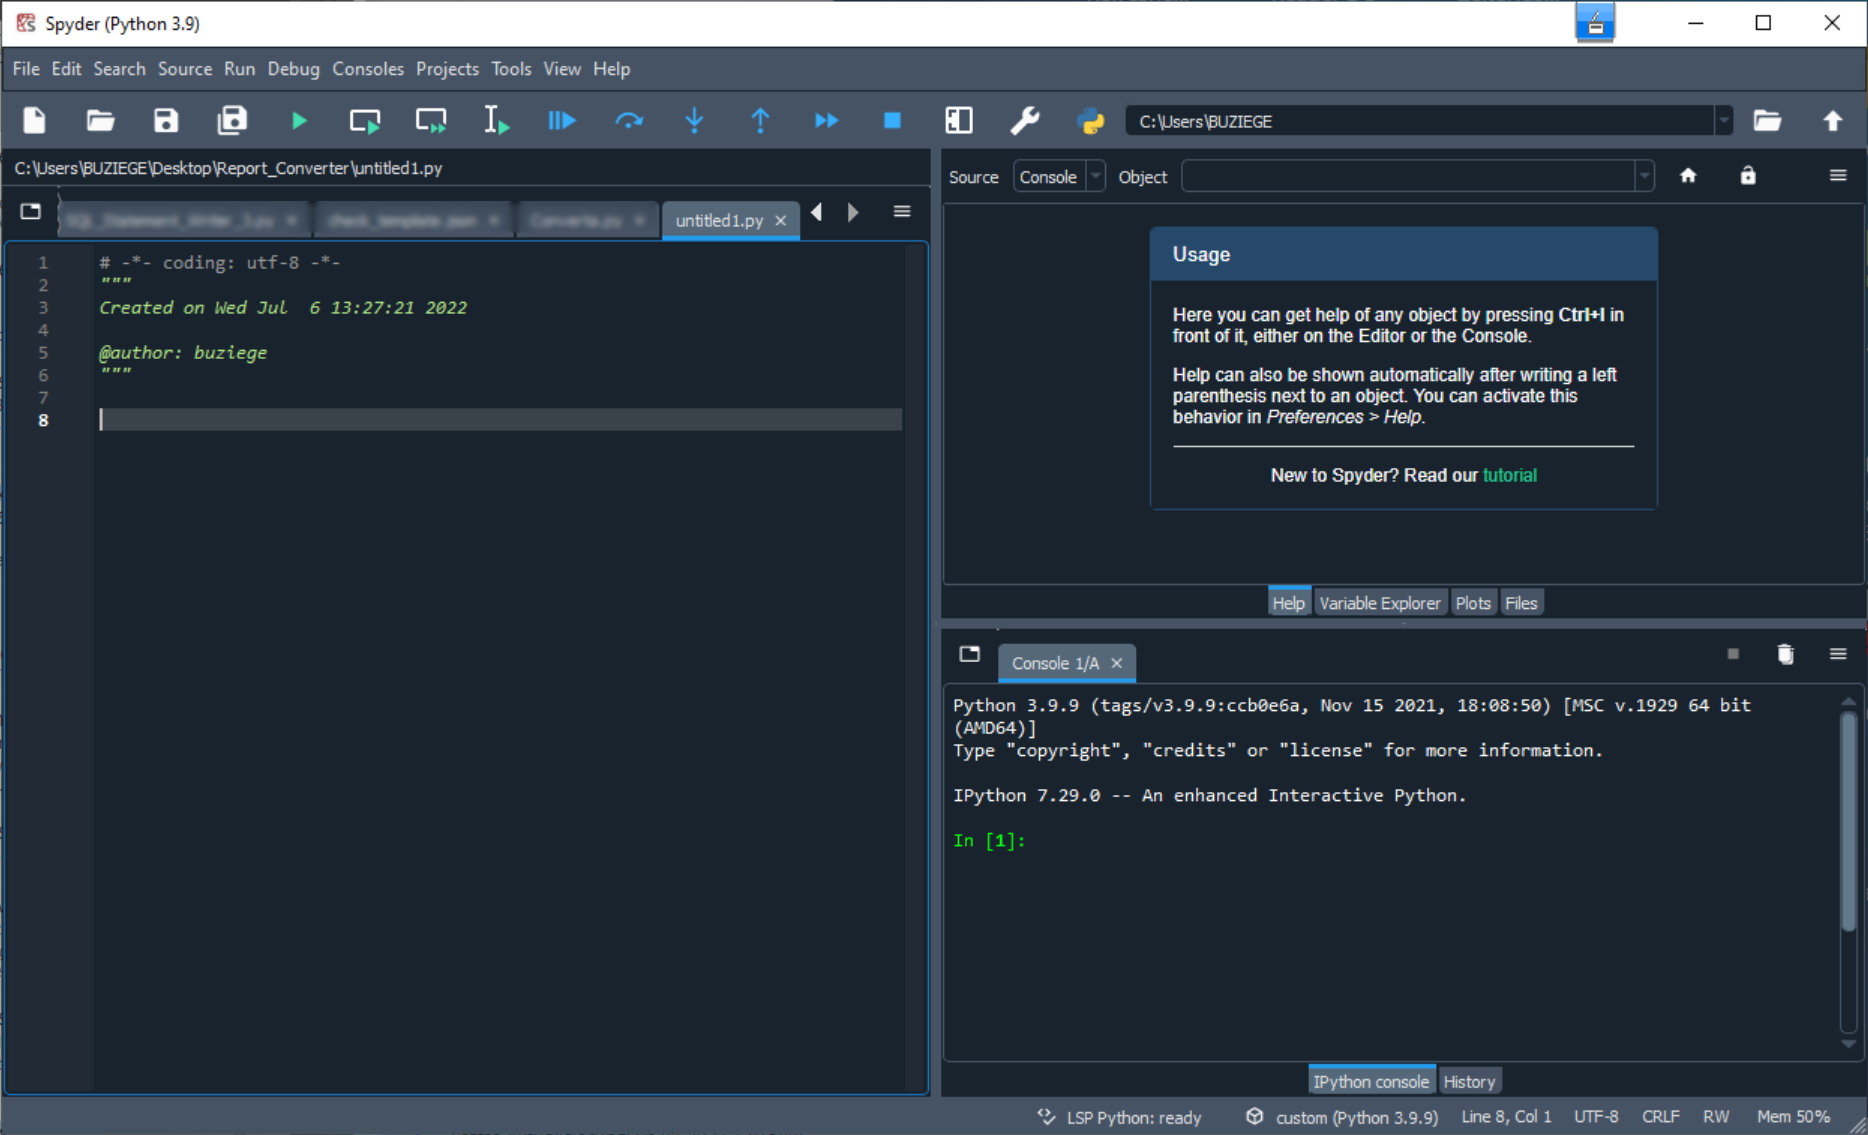
\includegraphics[width=\textwidth]{Pictures/Spyder5}
\end{center}

\end{frame}

\begin{frame}[fragile]
\frametitle{Python as a Calculator}

\begin{itemize}
\item Spyder5 runs an IPython kernel, this runs our programs
\item We can also use it as a calculator
\end{itemize}

\begin{lstlisting}[style=Python]
In [1]: 4*5.4
Out[1]: 21.6

In [2]: 4/12
Out[2]: 0.3333333333333333

In [3]: _*3
Out[3]: 1.0

'hello'
Out[4]: 'hello'
\end{lstlisting}

\end{frame}


\begin{frame}[fragile]
\frametitle{Python as a Calculator}

\begin{lstlisting}[style=Python]

In [1]: 4%2
Out[1]: 0

In [2]: 5%2 # Modulo
Out[2]: 1

In [3]: 3**3 # Power
Out[3]: 27

In [4]: 5//2
Out[4]: 2
\end{lstlisting}

By the way: \texttt{\#} indicates a comment

\end{frame}

\begin{frame}
\frametitle{Exercise 1}


\begin{itemize}
\item Start Spyder
\item Run some basic calculations in the Console window
\item Put them also in a Python file and run them from there using F5 and F9
\item What is the difference between using F5 or F9?
\end{itemize}
\end{frame}



\begin{frame}
\frametitle{Priority of Operators}

\begin{itemize}
\item Round brackets have highest priority
\item followed by Power
\item followed by multiplication and division
\item followed by addition and substraction
\end{itemize}

%\begin{block}{TODO4U:}
%$\Rightarrow$ Solve exercise sheet 1!
%\end{block}

\end{frame}

\begin{frame}[fragile]
\frametitle{Basic Input \& Output}

\lstinputlisting[style=Python]{Codes/Basic_IO.py}

\begin{itemize}
	\item Strings use either single or double quotation marks
	\item \lstinline[style=Python]{input()} only reads strings	
	\item If you need to process a number, you need to convert it 
	\item there are better ways than \lstinline[style=Python]{print()} for logging, but it works\ldots 
	\item f-Strings (last row) are recommended for mixed output!
	\end{itemize}
\end{frame}

\begin{frame}
\frametitle{Exercise 2}

\begin{itemize}
\item The formula to convert degrees Celsius to \newline degrees Fahrenheit is

\[  (c \times 1.8) + 32 \] with $c$ as the value in Celsius

\item Write some code that 

\begin{itemize}
	\item asks a celsius-value from the user
	\item converts it into Fahrenheit 
	\item stores the result in a variable
	\item prints the result using f-Strings
	\item Hint: to convert the string into a \newline floating-point number, use \texttt{float(<string>)}
	\end{itemize}

\end{itemize}
\end{frame}


\begin{frame}[fragile]
\frametitle{Basic Input \& Output - Raw Strings}

\begin{itemize}
	\item Certain characters need to be escaped
	\item A list is e.\,g. here: \url{https://www.w3schools.com/python/gloss_python_escape_characters.asp} 
	\item Raw strings can be used to prevent (most) processing, simply put an \enquote{r} before the string\footnote{A raw string must not end with a backslash}
	\end{itemize}

\lstinputlisting[style=Python]{Codes/rawStrings.py}


\end{frame}


\begin{frame}
\frametitle{Rules for Variables}

\begin{itemize}
\item must start with a letter or \textunderscore
\item Case-sensitivity: 'A' is not 'a'
\item For naming conventions see \url{https://realpython.com/python-pep8/}
\item Most important hint: let them speak for themselves: 'diameter' is good, 'd' is bad 
\end{itemize}
\end{frame}


\begin{frame}
\frametitle{Reserved Keywords}

The following  keywords are reserved and must not be used to name variables:

\begin{center}
\begin{tabular}{p{0.15\textwidth}p{0.15\textwidth}p{0.15\textwidth}p{0.15\textwidth}p{0.15\textwidth}}
and	&	as	&	assert	&	break	&	class	\\
continue	&	def	&	del	&	elif	&	else	\\
except	&	False	&	finally	&	for	&	from	\\
global	&	if	&	import	&	in	&	is	\\
lambda	&	None	&	nonlocal	&	not	&	or	\\
pass	&	raise	&	return	&	True	&	try	\\
while	&	with	&	yield	&		&		\\
\end{tabular}
\end{center}
\end{frame}



\subsection{Datatypes}

\begin{frame}
\frametitle{Datatypes}


\begin{itemize}
\item Integer (integer numbers)
\item Float (Floating point number)
\item Strings
\item Booleans
\item Complex numbers
\end{itemize}
\end{frame}

\begin{frame}
\frametitle{Integer}

\begin{itemize}
\item unlimited length
\item must not start with 0 if they shall represent decimal numbers 
\item Leading 0 by representation in hex-, binary- or Octal system:
\begin{description}
\item[\texttt{0b/0B}] binary
\item[\texttt{0x/0X}] hex
\item[\texttt{0o/0O}] octal
\end{description}
\item Functions \texttt{hex()}, \texttt{bin()}, \texttt{oct()} for conversions into string, are internally represented as decimal numbers 
\end{itemize}
\end{frame}

\begin{frame}
\frametitle{Float}

\begin{itemize}
	\item floating point numbers
	\item \texttt{3.1415927}
	\item \texttt{3.1e8}
	\item Hint: Not every floating point number can be represented \textit{exactly} (\enquote{Floating-Point Arithmetic}) 
	\item This can get tricky, if you compare numbers for equality
	\item \url{docs.python.org/3/tutorial/floatingpoint.html}

\end{itemize}
\end{frame}

\begin{frame}[containsverbatim]
\frametitle{Strings}

\begin{itemize}
\item Single or double quotes
\item For multiline strings:

\begin{itemize}
	\item Triple double or single quotes
	\item Alternatively backslash at the end of the line 
\end{itemize}

\item Python has numerous functions for strings, more on this later
\item Comments start with a hash \#
\end{itemize}


\begin{lstlisting}[style=Python]
a = "I am a string"

b = 'me too'

c = """I am 
as string as well """

# I am a comment
\end{lstlisting}


\end{frame}

\begin{frame}[containsverbatim]
\frametitle{Booleans}

\begin{itemize}
	\item Named after George Boole
	\item 1854: \enquote{An investigation into the Laws of Thought}
	\item Essence of modern computing
	\item Boolean operators or ($\cup$ ),  and ($\cap$ ), \texttt{not}
\end{itemize}

\begin{lstlisting}[language={Python}]
a = True
b = False 

a == b #False
a or b # True
a and b # False
a and not b # True
not a and b # False
\end{lstlisting}
\end{frame}



\begin{frame}[containsverbatim]
\frametitle{Type Conversions}

\begin{itemize}
\item Mixing strings and floats/integers requires explicit type conversion using the \lstinline[language={Python}]{str()} function
%\item Hint: pandas provides \lstinline[morekeywords={astype},language={Python}]{.astype(<Datatype>)} 
\item Use \texttt{int()} and \texttt{float()} to convert from string to number
\end{itemize}

\begin{lstlisting}[language={Python}]
>>> a + str(b)
'abc123'
>>> a+str(c)
'abc3.141'
>>> a*str(b)
Traceback (most recent call last):
  File "<stdin>", line 1, in <module>
TypeError: can't multiply sequence by non-int of type 'str'

>>> 'a' * 3
'aaa'

>>>3 * 'a'
'aaa'
\end{lstlisting}

%\begin{center}
%\fomh{$\Rightarrow$ Bitte Arbeitsblatt 2 bearbeiten!}
%\end{center}

\end{frame}

\subsection{Functions}


\begin{frame}
\frametitle{Functions}

\begin{itemize}
%\item Bereits bekannte Funktionen:  \lstinline[language={Python}]{id()} , \lstinline[language={Python}]{len()}  und \lstinline[language={Python}]{type()} 
\item Functions: named sequence of commands
\item Purpose: encapsule code for multiple calls
\item \textit{Can} take arguments as input, \textit{can} have return values
\item Define a new function as
\begin{itemize}
	\item Determine name
	\item Determine arguments
	\item Define function code
	\end{itemize}
\end{itemize}
\end{frame}


\begin{frame}
\frametitle{Built-in Functions}

\begin{tabular}{lllll}
abs	&	delattr	&	hash	&	memoryview	&	set	\\
all	&	dict	&	help	&	min	&	setattr	\\
any	&	dir	&	hex	&	next	&	slice	\\
ascii	&	divmod	&	id	&	object	&	sorted	\\
bin	&	enumerate	&	input	&	oct	&	staticmethod	\\
bool	&	eval	&	int	&	open	&	str	\\
breakpoint	&	exec	&	isinstance	&	ord	&	sum	\\
bytearray	&	filter	&	issubclass	&	pow	&	super	\\
bytes	&	float	&	iter	&	print	&	tuple	\\
callable	&	format	&	len	&	property	&	type	\\
chr	&	frozenset	&	list	&	range	&	vars	\\
classmethod	&	getattr	&	locals	&	repr	&	zip	\\
compile	&	globals	&	map	&	reversed	&	\textunderscore \textunderscore import \textunderscore \textunderscore	\\
complex	&	hasattr	&	max	&	round	&		\\
\end{tabular}
\end{frame}


%
%\begin{frame}[containsverbatim]
%\frametitle{Functions in C and Python}
%
%\lstinputlisting[language={C},caption={addTwoNumbers.c \ta{Codes/addTwoNumbers.c}}]{Codes/addTwoNumbers.c}\vspace*{-0.5em}
%
%\lstinputlisting[language={Python},caption={addTwoNumbers.py \ta{Codes/addTwoNumbers.py}}]{Codes/addTwoNumbers.py}
%
%\end{frame}


\begin{frame}[containsverbatim]
\frametitle{Simple Functions with any parameter}

\begin{itemize}
	\item \texttt{def} starts function definition
	\item do not forget \texttt{:} at the end of the \texttt{def} line
	\item indent the code inside the function using tabulator\footnote{Spyder expands it to four space characters}
	\item No input parameter in round brackets
	\item No return value (\texttt{void})
\end{itemize}

\lstinputlisting[language={Python},caption={funktion-01.py \ta{Codes/funktion-01.py}}]{Codes/funktion-01.py}

\begin{ausgabe}
Hello
\end{ausgabe}

\end{frame}

\begin{frame}[containsverbatim]
\frametitle{Simple Functions}
\framesubtitle{Empty Functions}

\begin{itemize}
\item \lstinline[language={Python}]{pass} is often used in the development process
\item Useful, when parts of the code are not ready, yet
\item without \lstinline[language={Python}]{pass} one gets \texttt{IndentationError: expected an indented block} error
\end{itemize}

\lstinputlisting[language={Python},caption={funktion-12.py \ta{Codes/funktion-12.py}}]{Codes/funktion-12.py}

\end{frame}





\begin{frame}[containsverbatim]
\frametitle{Functions with Arguments}

\begin{itemize}
	\item Function with one argument \texttt{text} 
	\item Error message, when argument is missing
\end{itemize}

\lstinputlisting[language={Python},caption={funktion-02.py \ta{Codes/funktion-02.py}}]{Codes/funktion-02.py}

\begin{ausgabe}
Hello World!
\end{ausgabe}

\end{frame}



\begin{frame}[containsverbatim]
\frametitle{Functions with Arguments}

\begin{itemize}
	\item Two arguments, \texttt{text} and \texttt{count}
\end{itemize}

\lstinputlisting[language={Python},caption={funktion-03.py \ta{Codes/funktion-03.py}}]{Codes/funktion-03.py}

\begin{ausgabe}

Hello!
Hello!Hello!Hello!

\end{ausgabe}

\end{frame}

\begin{frame}[containsverbatim]
\frametitle{Functions with Arguments}

\begin{itemize}
	\item Setting standard values for parameters
	\item Allows calling the function without parameters
\end{itemize}

\lstinputlisting[language={Python},caption={funktion-04.py \ta{Codes/funktion-04.py}}]{Codes/funktion-04.py}

\begin{ausgabe}
Hello CGNHello CGN
Hello!Hello!
Hello!Hello!Hello!
\end{ausgabe}

\end{frame}

\begin{frame}[containsverbatim]
\frametitle{Functions with return values}

\begin{itemize}
	\item Functions can return values for further processing
\end{itemize}

\lstinputlisting[language={Python},caption={funktion-05.py \ta{Codes/funktion-05.py}}]{Codes/funktion-05.py}

\begin{ausgabe}
HuhuHuhu
\end{ausgabe}

\end{frame}


\begin{frame}
\frametitle{Exercise 3}

\begin{itemize}
\item Use the code from the temperature conversion 
\item create a function for the conversion from Celsius to Fahrenheit
\item Call the function multiple times
\end{itemize}
\end{frame}

\begin{frame}[containsverbatim]
\frametitle{Solution for Exercise 3}


\lstinputlisting[language={Python},caption={c2f-function \ta{Codes/funktion-05.py}}]{Codes/c2f_function.py}


\end{frame}


\begin{frame}[containsverbatim]
\frametitle{Info: Functions with multiple return values}

\begin{itemize}
	\item Functions can have more than one return value
	\item Function then return tuples, an unmutuable list of values\footnote{more on this later}
	\item Dealing with the tuple is called \enquote{Unpacking}
	\item Remark: Parameter \texttt{sep} in the example is a parameter \newline of the \lstinline[language={Python}]{print()}  function
\end{itemize}

\lstinputlisting[language={Python},caption={funktion-06.py \ta{Codes/funktion-06.py}}]{Codes/funktion-06.py}

\vspace*{-1em}
\begin{ausgabe}
2>HuhuHuhu
\end{ausgabe}
\end{frame}

\begin{frame}
\frametitle{Info: Functions with variable count of arguments}

\begin{itemize}
\item Parameter with *: variable count of arguments
\item Parameter with **: variable count of key-value arguments
\end{itemize}

\lstinputlisting[language={Python},caption={funktion-08.py \ta{Codes/funktion-08.py}}]{Codes/funktion-08.py}

\lstinputlisting[language={Python},caption={funktion-09.py \ta{Codes/funktion-09.py}}]{Codes/funktion-09.py}

\end{frame}


\subsection{Flow control}

\begin{frame}
\frametitle{Flow control}

\begin{itemize}
\item Input \& Output \checkmark
\begin{itemize}
	\item input
	\item print
\end{itemize}

\item Branching
\begin{itemize}
	\item if else elif
\end{itemize}

\item Loops
\begin{itemize}
	\item for
	\item while
\end{itemize}

\end{itemize}
\end{frame}

\begin{frame}[containsverbatim]
\frametitle{Branching}

\begin{itemize}
\item \lstinline[language={Python}]{if <condition>:}
\end{itemize}

\lstinputlisting[language={Python},caption={if-01.py \ta{Codes/if-01.py}} ]{Codes/if-01.py}

\begin{ausgabe}
Longer than 8 characters!
\end{ausgabe}
\end{frame}

\begin{frame}[containsverbatim]
\frametitle{Branching}

\begin{itemize}
\item There is no \texttt{switch()} in Python < 3.10\footnote{From 3.10 there is \texttt{match}/\texttt{case}, see \url{stackoverflow.com/questions/11479816/}}
\item \lstinline[language={Python}]{if} statements can be used multiple times
\item maybe not the most pythonic approach
\end{itemize}

\lstinputlisting[language={Python},caption={if-02.py \ta{Codes/if-02.py}}]{Codes/if-02.py}

\begin{ausgabe}
Köln: Shorter or equal to 8 characters!
Düsseldorf: Longer than 8 characters!
\end{ausgabe}
\end{frame}


\begin{frame}[containsverbatim]
\frametitle{Branching}

\begin{itemize}
\item more \enquote{pythonic}:  \lstinline[language={Python}]{else:}
\end{itemize}

\lstinputlisting[language={Python},caption={if-03.py \ta{Codes/if-03.py}}]{Codes/if-03.py}

\begin{ausgabe}
Köln: Shorter or equal to 8 characters!
Düsseldorf: Longer than 8 characters!
\end{ausgabe}

\end{frame}

\begin{frame}[containsverbatim]
\frametitle{Branching}

\begin{itemize}
\item Nesting von \lstinline[language={Python}]{if <condition>: else:} leads to confusing code
\end{itemize}

\lstinputlisting[language={Python},caption={if-04.py \ta{Codes/if-04.py}}]{Codes/if-04.py}

\begin{ausgabe}
Köln: Shorter or equal 5 chars!
Berlin: Longer than 5, shorter than 8
Düsseldorf: Longer than 8 chars!
\end{ausgabe}

\end{frame}

\begin{frame}[containsverbatim]
\frametitle{Branching}

\begin{itemize}
\item \lstinline[language={Python}]{if <condition>: else:} can be shortened to \lstinline[language={Python}]{elif:} 
\end{itemize}

\lstinputlisting[language={Python},caption={if-05.py \ta{Codes/if-05.py}}]{Codes/if-05.py}

\begin{ausgabe}
Köln: Shorter or equal 5 chars!
Berlin: Longer than 5, shorter than 8
Düsseldorf: Longer than 8 chars!
\end{ausgabe}


\end{frame}


\begin{frame}[containsverbatim]
\frametitle{Loops}
\framesubtitle{\lstinline[language={Python}]{for}}

\begin{itemize}
\item \lstinline[language={Python}]{for} loops iterate over a sequence
\item sequence can be a string, a liste, etc. 
\item \lstinline[language={Python}]{range(start, end, stepsize=1)} creates numerical sequence from \texttt{start} until below (!) \texttt{end} with step size \texttt{stepsize}
\end{itemize}

\lstinputlisting[language={Python},caption={for-01.py \ta{Codes/for-01.py}}]{Codes/for-01.py}

\end{frame}


\begin{frame}[containsverbatim]
\frametitle{Loops}
\framesubtitle{\lstinline[language={Python}]{while}}

\begin{itemize}
\item \lstinline[language={Python}]{while} loop runs, until condition is not fulfilled anymore
\end{itemize}

\lstinputlisting[language={Python},caption={while-01.py \ta{Codes/while-01.py}}]{Codes/while-01.py}

\end{frame}

\begin{frame}[containsverbatim]
\frametitle{Loops}
\framesubtitle{\lstinline[language={Python}]{break} and \lstinline[language={Python}]{continue}}

\begin{itemize}
\item \lstinline[language={Python}]{break} and \lstinline[language={Python}]{continue} influence loops
\item \lstinline[language={Python}]{break} can e.\,g. be used to exit a loop 
\end{itemize}

\lstinputlisting[language={Python},caption={while-02.py \ta{Codes/while-02.py}}]{Codes/while-02.py}

\end{frame}


\subsection{File-Operations}

\begin{frame}[containsverbatim]
\frametitle{File-Operations}

\begin{itemize}
\item \texttt{open()} opens file for read/write access
\item two parameters:

\begin{description}
\item[Path] Path to the file
\item[Mode] Read, Write, Binary, Text
\end{description}
\end{itemize}

\begin{lstlisting}[language=Python,caption={Simple example for \texttt{write()}}]
f = open('u:/hello.txt', 'w')
f.write("Hello World!")
f.close()
\end{lstlisting}

Not optimal, in case of errors the file-handle might remain open! The file is not usable by other applications.
\end{frame}


\begin{frame}[containsverbatim]
\frametitle{File-Operations}

Improved version, uses \enquote{Context manager}, closes file handle in each situation

\begin{lstlisting}[language=Python,caption={Improved example for \texttt{write()}}]
with open('r:/hello.txt', 'w') as f:
    f.write("Hello World!")
\end{lstlisting}

Hint: Context managers are also very useful when dealing with SQL databases.

\end{frame}

\begin{frame}
\frametitle{Exercise 4: Files and Branching}


\begin{itemize}
\item Ask the user to input a number
\item If the number < 0 write \enquote{Hello} to a text file
\item If the number > 0 write \enquote{World} to a text file
\item If the number = 0 write \enquote{Foobar} to a text file
\item Open the file and printout the file on the screen
\item Delete the created file afterwards
\end{itemize}
\end{frame}

\begin{frame}[containsverbatim]
\frametitle{File-Operations}

Read-/Write- parameters

\begin{description}
\item [r] Read; Error, when file is not present
\item [r+] Read and Write
\item [a+] Read and append, file is created if not existent
\item [x] Creates file, error if file exists
\item [a] Append; creates file if not existent, appends at the end
\item [w] Write; creates file if not existent; overwrite, if file exists
\end{description}

Content format

\begin{description}
\item[t] for text files
\item[b] for binary files (images, zip, etc)
\end{description}

\end{frame}

\begin{frame}[containsverbatim]
\frametitle{File-Operations}

\begin{lstlisting}[language=Python,caption={Read a complete file}]
with open('r:/hello.txt', 'rt') as file:  
    print(file.read())
\end{lstlisting}

\begin{lstlisting}[language=Python,caption={Row-wise reading a file}]
with open('r:/hello.txt', 'rt') as file:  
    for line in file:
        print(x)
\end{lstlisting}

\end{frame}



\begin{frame}[containsverbatim]
\frametitle{File-Operations}
\framesubtitle{Deleting files}

\begin{lstlisting}[language=Python,caption={Deleting a file}]
import os

if os.path.exists('r:/hello.txt'):
    os.remove('r:/hello.txt')
else:
    print("File does not exist!")   
\end{lstlisting}

\end{frame}

\subsection{Ranges and Strings}



\begin{frame}[containsverbatim]
\frametitle{The \texttt{range()} Function}

\begin{itemize}
\item \texttt{range()} function creates a sequence of numbers via \texttt{generator}$\Rightarrow$ see next slide
\item Three parameters maximum : \texttt{start}, \texttt{stop} and \texttt{step}
\item \texttt{range(<stop>)} with one parameter,  \texttt{range(0,<stop>,1)} implicitly
\item \texttt{range(<start>, <stop>)} with two parameters, \texttt{<start>,<stop>,1)} implicitly 
\item \texttt{range(<start>,<stop>,<step>)} with three parameters
\item Important: \texttt{<start>} is inclusive, \texttt{<stop>} not!!!
\item \texttt{range(0,10)} runs from 0 to 9
\end{itemize}
\end{frame}

\begin{frame}[containsverbatim]
\frametitle{Examples for \texttt{range()}-Function}

\lstinputlisting[basicstyle=\ttfamily\tiny,language={Python},caption={range\textunderscore beispiel.py \ta{codes/range_beispiel.py}}]{codes/range_beispiel.py}

\begin{ausgabe}
1: 0	1 1	1 2	1 3	1 4	1 5	1 6	1 7	1 8	1 9
2: 2	2 3	2 4	2 5	2 6	2 7	2 8	2 9		
3: 2	3 4	3 6	3 8						
4: 10	4 8	4 6	4 4	4 2	4 0	4 -2	4 -4	4 -6	4 -8
\end{ausgabe}

\end{frame}


\subsection{Sequential Datatypes}

\begin{frame}
\frametitle{Sequential Datatypes aka: for i in whatever}

\begin{itemize}
\item Sequential Datatypes = Datatypes that store elements sequentially

\begin{description}
\item[Strings] contain characters only
\item[Lists] different objects possible, mutuable (changeable)
\item[Tuple] different objects possible, not mutuable \newline (not changeable)
\end{description}
\item Identical methods for the access: \lstinline[language={Python}]{object[<number>]} to access a specific element, \lstinline[language={Python}]{len()} for the length, Slicing-Notation
\end{itemize}
\end{frame}

%\begin{frame}
%\frametitle{Strings}
%
%\begin{itemize}
%\item Single or double quotation marks
%\item Notation mit \texttt{'''} resp. \texttt{''''''} used in documentations, allows multi-line strings
%\end{itemize}
%\end{frame}
%
%\begin{frame}
%\frametitle{List of Escape-Sequences (Extract)}
%
%\begin{itemize}
%	\item Various characters must be  \enquote{escaped} 
%	\item Complete list here: \url{docs.python.org/3/reference/lexical_analysis.html}
%\end{itemize}
%
%\begin{center}
%\begin{tabular}{c|l}
%Character & Description \\ \toprule
%\textbackslash \textbackslash & Backslash \\
%\textbackslash t & Tabulator \\
%\textbackslash n & Linebreak \\ \bottomrule
%\end{tabular}
%\end{center}
%
%\begin{itemize}
%	\item Prevent expansion by \enquote{raw} statement:
%	\item \lstinline[language={Python}]{print(r'Hello\\nWorld')}, used e.\,g. with regular expressions
%\end{itemize}
%
%\end{frame}

\begin{frame}[containsverbatim]
\frametitle{String Functions}

\begin{itemize}
\item Numerous string-functions are available, see \url{docs.python.org/3/library/stdtypes.html#text-sequence-type-str} 
\item Length of a string using \lstinline[language={Python}]{len(<String>)}
\item Upper- or lowercase a string with \lstinline[language={Python}]{upper(<String>)} and \lstinline[language={Python}]{lower(<String>)}
\item \lstinline[language={Python}]{index(<String>)}, \lstinline[language={Python}]{find(<String>)} and \lstinline[language={Python}]{replace(<String>)}
\item \lstinline[language={Python}]{startswith(<String>)} and \lstinline[language={Python}]{endwith(<String>)}
\item \lstinline[language={Python}]{split(<String>)} and \lstinline[language={Python}]{strip(<String>)}
\end{itemize}

\end{frame}



\begin{frame}[containsverbatim]
\frametitle{Lists}

\begin{itemize}
\item Lists contain arbitrary objects
\item Square brackets, elements separated by comma
\item first element is \texttt{listname[0]}
\item Can be nested
\item Can be changed at runtime $\Rightarrow$ \enquote{mutuable}
\end{itemize}

\begin{lstlisting}[language={Python}]
abc = ['a', 'b', 'c', 3.1234]
efg = [1, 2, [1, 2, 3], 3, 4]
\end{lstlisting}

\end{frame}

\begin{frame}
\frametitle{Tuples}

\begin{itemize}
\item Round brackets, can be left out
\item Recommendation: do not leave them out
\item Immutable, objects cannot be changed after creation
\item can be unpacked via multi-assignment: \lstinline[language={Python}]{a, b, c = (1, 2, 3)}
\item hint: switch two numbers by \lstinline[language={Python}]{a, b = b, a}
\end{itemize}
\end{frame}

\begin{frame}
\frametitle{Indexing Sequential Datatypes}

\begin{itemize}
	\item Two ways of indexing: from \(0 \text{ to } n-1\) and \(-n \text{ to } -1\)
\end{itemize}

\begin{center}
\begin{tabular}{r|c|c|c|c|c|c|c|c|c|c|c|}
Index & -11 & -10 & -9 & -8 & -7 & -6 & -5 & -4 & -3 & -2 & -1 \\ \toprule
&H&e&l&l&o& &W&o&r&l&d \\ \toprule
Index & 0 & 1 & 2 & 3 & 4 & 5 & 6 & 7 & 8 & 9 & 10 \\ \toprule
\end{tabular}
\end{center}

\end{frame}

\begin{frame}[containsverbatim]
\frametitle{Slicing}

\begin{itemize}
\item Slicing = very powerful, especially for strings
\item two parameters, start and stop, separated by \texttt{:}, both are optional
\item third parameter: step size
\end{itemize}\vspace*{0em}

\begin{lstlisting}[language={Python}]
>>> a = 'Hello World'
>>> a[:]
'Hello World'
>>> a[1:-1]
'ello Worl'
>>> a[1:-5]
'ello '
>>> a[::1]
'Hello World'
>>> a[::2]
'HloWrd'
>>> a[1:-1:3]
'eoo'
>>>a[::-1]
\end{lstlisting}

\end{frame}

\begin{frame}
\frametitle{Exercise 5: String manipulation}

\begin{itemize}
\item Ask the user to input a file name, or alternatively: use the filenames in a directory of your choice
\item print the filename without the file extension as well as the file extension separately
\end{itemize}
\end{frame}

\begin{frame}
\frametitle{Dictionaries}

\begin{itemize}
\item Dictionaries = Associative fields, maps, hashes
\item consist of Key-Value pairs, for each (\enquote{Key}) a (\enquote{Value}) is assigned
\item each key must only exist once in each dict
\item can arbitrarily grow and shrink
\item all immutable objects can be keys: strings, floats, integers, tuples, but no lists or dictionaries
\item Dictionaries can be nested (well, if you ever need this, think again\ldots)
\end{itemize}
\end{frame}

\begin{frame}[containsverbatim]
\frametitle{Dictionaries}

\pypy{dict-01.py}{Codes/dict-01.py}

\begin{ausgabe}
Tree
Januar
\end{ausgabe}

\end{frame}


\begin{frame}[containsverbatim]
\frametitle{Accessing a Dictionary}

\vspace*{-0.5em}\pypy{dict-04.py}{Codes/dict-04.py}

\vspace*{-0.5em}\begin{ausgabe}
dict_keys([1, 2, 3])
dict_values(['one', 'two', 'three'])
dict_items([(1, 'one'), (2, 'two'), (3, 'three')])
None
three
1 one
2 two
3 three
\end{ausgabe}

\end{frame}



\begin{frame}[containsverbatim]
\frametitle{Functions for Dictionaries (Selection)}

\begin{description}
\item[\texttt{clear()}] deletes all entries
\item[\texttt{copy()}] creates a flat copy
\item[\texttt{keys()}] set of all keys
\item[\texttt{pop()}] removes key and its value from dict
\item[\texttt{update()}] adds dict2 to dict, overwrites values eventually
\item[\texttt{popitem()}] removes arbitrary key-value combination from dict, KeyError if dict is empty. Important: \enquote{arbitrary} $\not=$ {random}!
\end{description}

\end{frame}



\section{pandas}

\begin{frame}
\frametitle{pandas}

\begin{itemize}
	\item A Python library for data wrangling and management
	\item Invented by Wes McKinney during his time at AQR Capital Management
	\item In his own words:
\enquote{I tell them that it enables people to analyze and work with data who are not expert computer scientists,} he says. \enquote{You still have to write code, but it’s making the code intuitive and accessible. It helps people move beyond just using Excel for data analysis.}\footnote{\url{qz.com/1126615/the-story-of-the-most-important-tool-in-data-science/}}
\end{itemize}

\end{frame}



\begin{frame}[containsverbatim]
\frametitle{Das SciPy Framework}
\framesubtitle{~}

\texttt{pandas} is just a piece among many:\vspace*{1em}

\begin{description}
\item[NumPy] Matrices, vectors, algorithms
\item[IPython] Matlab/Mathematica-like environment
\item[Matplotlib] Scientific Plotting, Basis for \texttt{seaborn} library
\item[SymPy] Symbolic mathematics
\item [\ldots] etc, etc
\end{description}\vspace*{0.5em}

We only focus on \texttt{pandas} today:

\begin{lstlisting}
import pandas as pd
\end{lstlisting}

\end{frame}

\begin{frame}
\frametitle{Series and DataFrames}

\begin{itemize}
\item central data structures in  \texttt{pandas}: \texttt{series} and \texttt{dataframes}
\item quite similar to dataframes in R
\item Definition \enquote{Series}: a vector with data of the same type and an index
\item Definition \enquote{Dataframe}: matrix from various series, the series can have different data types haben but they share the same index
\end{itemize}
\end{frame}

\begin{frame}
\frametitle{Series und DataFrames}

\begin{figure}
\begin{center}
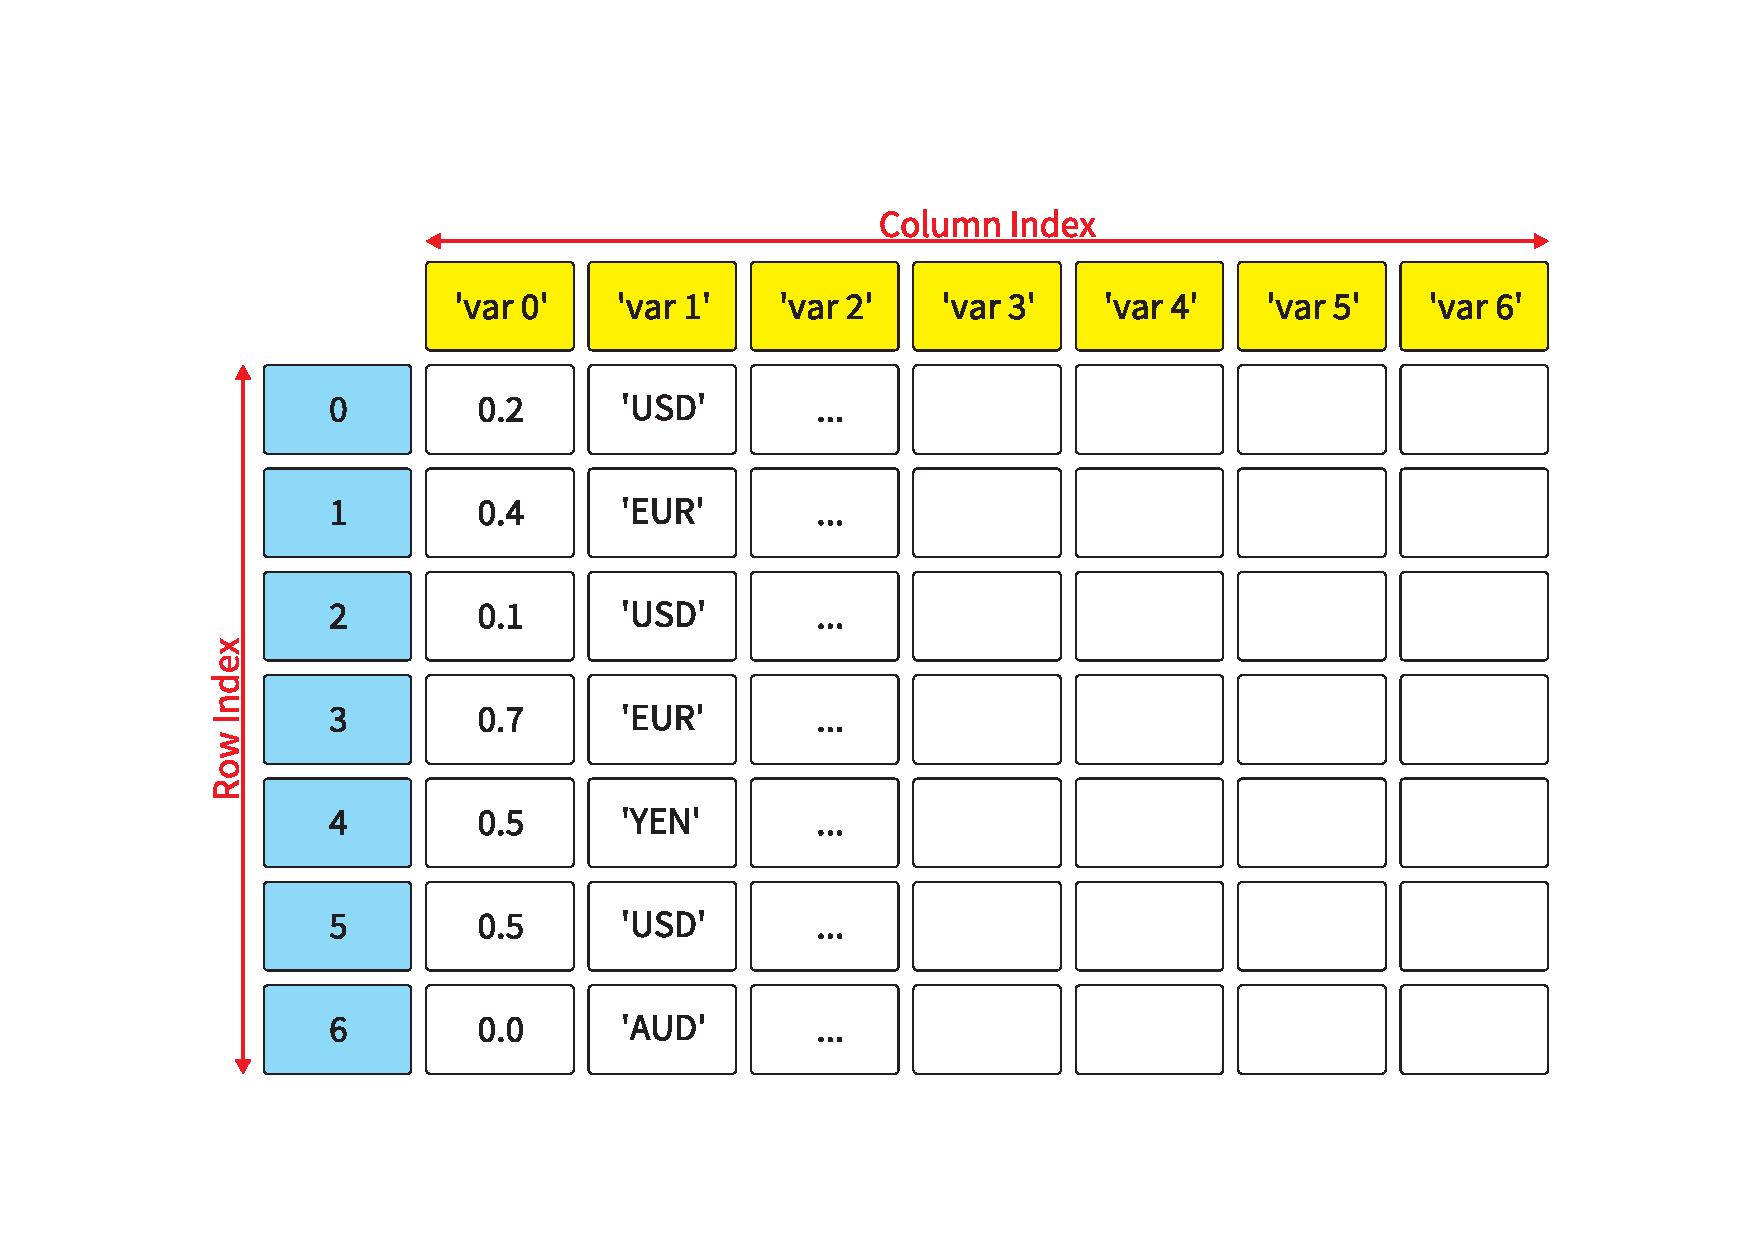
\includegraphics[trim=50mm 55mm 45mm 55mm,width=0.8\textwidth]{Pictures/SeriesFrames.pdf}
\end{center}
\end{figure}

\end{frame}


\begin{frame}[containsverbatim]
\frametitle{Manual Creation of pandas Objects}
\framesubtitle{~}

\begin{itemize}
	\item pandas-objecs \textit{can} be created manually
	\item normally not used, data is usually loaded from files/databases
\end{itemize}

\begin{lstlisting}
import pandas as pd

d = pd.DataFrame({'A': ['A0','A1','A2','A3'], 
	'Key': ['K0','K1','K2','K4']})
a = pd.Series([1,2,3,4,5,6,7,8,9,10])
b = pd.Series(['A','C','D','B','F','G','I','K','L','P'])
df = pd.concat([a,b], axis=1)
# alternatively
df = pd.DataFrame({'a': a,'b':b})
df = a.to_frame().join(b.to_frame())
df = pd.DataFrame(data=dict(a=a, b=b))
\end{lstlisting}
\end{frame}

\begin{frame}
\frametitle{Daten einlesen}
\framesubtitle{~}

\begin{itemize}
	\item various functions to read files
\end{itemize}

\begin{center}
\begin{tabular}{ll} \toprule
Befehl & Beschreibung \\ \midrule
read\textunderscore pickle &reads Pickle objects\\
read\textunderscore table & table-like formats \\
read\textunderscore csv & Comma-Separated Values  \\
read\textunderscore fwf & fixed-width formats \\
read\textunderscore clipboard & clipboard \\
read\textunderscore excel & Excel-files\\ \bottomrule
\end{tabular}\vspace*{-0.35em}
\end{center}

other commands for HTML, JSON, HDF5, \ldots
\end{frame}



\begin{frame}[containsverbatim]
\frametitle{Reading CSV}
\framesubtitle{~}

\begin{itemize}
\item \enquote{CSV}: Comma-Separated Value
\item CSV is not a unique format
\begin{itemize}
	\item Column-separator
	\item Decimal-separator
	\item Text Encoding
\end{itemize}
\item Specifications: \url{http://pandas.pydata.org/pandas-docs/stable/generated/pandas.read_csv.html}
\begin{description}
\item[sep] Column-separator
\item[thousands] seperator for thousands
\item[encoding] Encoding
\item [decimal]  Decimal-separator
\item [converters] converters=\{'A': str\} for explicit conversion to a format
\end{description}
\end{itemize}
\end{frame}

\begin{frame}
\frametitle{Reading Excel}

\begin{itemize}
\item \lstinline[language={Python}]{pd.read_excel()} to read XLSX-files (!) \item Documentation: \url{http://pandas.pydata.org/pandas-docs/stable/generated/pandas.read_excel.html}
\item Export to Excel using \lstinline[language={Python}]{pd.to_excel()}
\item Remarks:
\begin{itemize}
	\item Excel-Export is way slower than CSV-Export
	\item Export of well-formatted Excel is possible but takes effort
	\item One can even control Excel via COM (Common Object Model)
\end{itemize}
\end{itemize}
\end{frame}

\begin{frame}[fragile]
\frametitle{DataFrames bearbeiten}
\framesubtitle{Exploratory Data Analysis}

\begin{itemize}
	\item We use \texttt{Northwind} data as an example
	\item First task after loading: check data consistency
\end{itemize}

\begin{lstlisting}[language={Python}]
customers = pd.read_excel('Northwind.xlsx', sheetname = 'Customers')

print(len(customers))     # number of rows
print(customers.head()) # first five rows
print(customers.tail())   # last five rows
print(list(customers))    # list of columns
\end{lstlisting}
\end{frame}


\begin{frame}
\frametitle{Aufgabe}


\begin{itemize}
\item Read the files \texttt{Bestandsdaten.csv}, \texttt{Bestandsdaten\textunderscore Vortag.csv}  and \texttt{Bewertung.xlsx} 
\item Check the data using the functions from last slide
\item Export the data to HTML, which columns could be used to connect the data sets with eachother?
\end{itemize}
\end{frame}

\begin{frame}[fragile]
\frametitle{Pandas Dataframe Operations}
\framesubtitle{Selection and Filtering I}

\begin{itemize}
	\item pandas has advanced methods for selecting, filtering and transforming data 
\item Select only specific columns

\lstinline[language={Python}]{df = df[['colA', 'colB']]}

\item Select the top two rows (Index starting at 0)

\lstinline[language={Python}]{df.iloc[:1]}

\item Select only those rows where one row > 50

\lstinline[language={Python}]{df[df['colA'] > 50]}
\end{itemize}
\end{frame}

\begin{frame}[fragile]
\frametitle{Pandas Dataframe Operations}
\framesubtitle{Selection and Filtering II}

\begin{itemize}
\item Select only those rows where value is between two values

\lstinline[language={Python}]{df[(df['colA'] > 50) | (df['colA'] < 500)]}

\item Select rows that \textbf{do not} have a certain value

\lstinline[language={Python}]{df[~(df['colA'] == 'HelloWorld')]}

\item Select rows, where column b is either value 'A' or 'B' 

\lstinline[language={Python}]{df = df[ (df['b'] == 'A') | (df['b'] == 'I')]}

\item Use alternatively  \lstinline[language={Python}]{isin()}

\lstinline[language={Python}]{df = df[df['b'].isin(['A','I'])]}

\item or the opposite

\lstinline[language={Python}]{df = df[~df['b'].isin(['A','I'])]}

\item More here: \url{http://chrisalbon.com/python/pandas_indexing_selecting.html}

\end{itemize}
\end{frame}


\begin{frame}[containsverbatim]
\frametitle{Apply functions to \texttt{pandas} columns}

\lstinputlisting[language={Python}]{Codes/pandas-funktional-01.py}

\begin{ausgabe}
  Key   Name Nachname
0  K0   anna     Anna
1  K1  bernd    Bernd
2  K2  cesar    Cesar
3  K4   dana     Dana
\end{ausgabe}

\end{frame}


\begin{frame}[fragile]
\frametitle{Mapping I}

\begin{itemize}
	\item Similar to Excel's \texttt{vlookup()} function
	\item Example: \texttt{countries} is a key-value dictionary
	\item \texttt{country} column in the dataframe is used as key in the dictionary, a new column is created
\end{itemize}

\lstinputlisting[language={Python}]{Codes/mapping-01.py}

\end{frame}

\begin{frame}[fragile]
\frametitle{Mapping II}

\begin{itemize}
	\item \texttt{map()} can also be used to make simple calculations
	\item keyword here is \enquote{lambda} $\Rightarrow$ anonymous function	
\end{itemize}

\lstinputlisting[language={Python}]{Codes/mapping-02.py}

\end{frame}

\begin{frame}[fragile]
\frametitle{Pandas Dataframe Operations}
\framesubtitle{Merge and Join}

\begin{itemize}
\item \texttt{merge()} SQL-like merging of datasets
\item useful to combine data
\item Supports the following join types:
\begin{itemize}
	\item Left
	\item Right
	\item Inner
	\item Full Outer
\end{itemize}
\item \texttt{join()} is a special alias for \texttt{merge()},  works on \newline the index, not the columns
\end{itemize}

\end{frame}

\begin{frame}[fragile]
\frametitle{Pandas Dataframe Operations}
\framesubtitle{Merge and Join}

\begin{itemize}
	\item Standard-command for \texttt{merge()}
\end{itemize}

\begin{lstlisting}
leftDataFrame.merge(rightDataFrame, how='inner', 
on=None, left_on=None, right_on=None, left_index=False, 
right_index=False, sort=False, suffixes=('_x', '_y'), 
copy=True, indicator=False)
\end{lstlisting}

\textbf{Workflow}

\begin{enumerate}
\item define other dataset
\item define type of merge
\item define keys for the merger
\end{enumerate}

\end{frame}


\begin{frame}
\frametitle{Merging}
\framesubtitle{Inner Join}

\begin{itemize}
\item Select all data, that is in A \textbf{and} B
\end{itemize}

\begin{center}
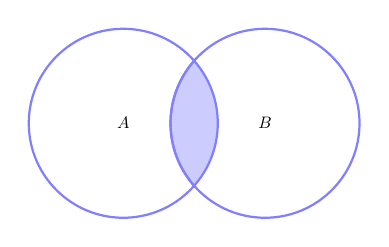
\begin{tikzpicture}[scale=0.6, every node/.style={scale=0.6}]
    \begin{scope}
        \clip \firstcircle;
        \fill[filled] \secondcircle;
    \end{scope}
    \draw[outline] \firstcircle node {$A$};
    \draw[outline] \secondcircle node {$B$};
    %\node[anchor=south] at (current bounding box.north) {$A \cap B$};
\end{tikzpicture}
\end{center}

{\footnotesize
\begin{columns}
\begin{column}{0.3\textwidth}
left \\
\begin{tabular}{c|cc} \toprule
   & A  &  Key \\ \midrule
0 & A0 &  K0 \\
1 & A1 &  K1 \\ 
2 & A2 &  K2 \\
3 & A3 &  \textcolor{red}{K4} \\ \bottomrule
\end{tabular}
\end{column}
\begin{column}{0.3\textwidth}
right \\
\begin{tabular}{c|cc} \toprule
   &  B   & Key \\ \midrule
0 &  B0 & K0 \\
1 &  B1 & K1 \\ 
2 &  B2 & K2 \\
3 &  C3 & \textcolor{red}{K5} \\ \bottomrule
\end{tabular}\end{column}
\begin{column}{0.3\textwidth}
merged \\
\begin{tabular}{c|ccc} \toprule
   & A  & B   & Key \\ \midrule
0 & A0 & B0 & K0 \\
1 & A1 & B1 & K1 \\ 
2 & A2 & B2 & K2 \\ \bottomrule
\end{tabular} \\
\vspace*{1.5em}
\end{column}
\end{columns}}


\end{frame}

\begin{frame}
\frametitle{Merging}
\framesubtitle{Left Join}

\begin{itemize}
\item Select all data in A, get data from B if available
\end{itemize}

\begin{center}
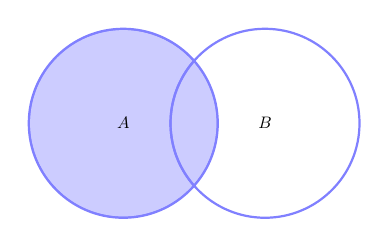
\begin{tikzpicture}[scale=0.6, every node/.style={scale=0.6}]
    \begin{scope}
        \clip \firstcircle;
        \draw[filled] \firstcircle node {$A$}
                                     \secondcircle;
    \end{scope}
    \draw[outline] \firstcircle
                   \secondcircle node {$B$};
    %\node[anchor=south] at (current bounding box.north) {$A - B$};
\end{tikzpicture}
\end{center}

{\footnotesize
\begin{columns}
\begin{column}{0.3\textwidth}
left \\
\begin{tabular}{c|cc} \toprule
   & A  &  Key \\ \midrule
0 & A0 &  K0 \\
1 & A1 &  K1 \\ 
2 & A2 &  K2 \\
3 & A3 &  \textcolor{red}{K4} \\ \bottomrule
\end{tabular}
\end{column}
\begin{column}{0.3\textwidth}
right \\
\begin{tabular}{c|cc} \toprule
   &  B   & Key \\ \midrule
0 &  B0 & K0 \\
1 &  B1 & K1 \\ 
2 &  B2 & K2 \\
3 &  C3 & \textcolor{red}{K5} \\ \bottomrule
\end{tabular}\end{column}
\begin{column}{0.3\textwidth}
merged \\
\begin{tabular}{c|ccc} \toprule
   & A  & B   & Key \\ \midrule
0 & A0 & B0 & K0 \\
1 & A1 & B1 & K1 \\ 
2 & A2 & B2 & K2 \\ \bottomrule
3 & A3 & NaN & K4 \\ \bottomrule
\end{tabular} \\
\vspace*{0.4em}
\end{column}
\end{columns}}

\end{frame}

\begin{frame}
\frametitle{Merging}
\framesubtitle{Right Join}

\begin{itemize}
\item Select all data in B, get data from A if available
\end{itemize}

\begin{center}
% Right Join
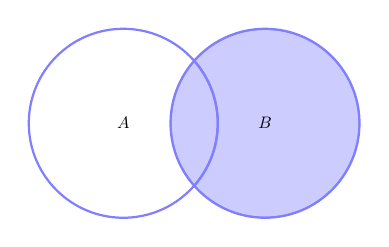
\begin{tikzpicture}[scale=0.6, every node/.style={scale=0.6}]
    \begin{scope}
        \clip \secondcircle;
        \draw[filled] \firstcircle \secondcircle node {$B$};
    \end{scope}
    \draw[outline] \firstcircle node {$A$}
                   \secondcircle;
    %\node[anchor=south] at (current bounding box.north) {$B - A$};
\end{tikzpicture}

\end{center}

{\footnotesize
\begin{columns}
\begin{column}{0.3\textwidth}
left \\
\begin{tabular}{c|cc} \toprule
   & A  &  Key \\ \midrule
0 & A0 &  K0 \\
1 & A1 &  K1 \\ 
2 & A2 &  K2 \\
3 & A3 &  \textcolor{red}{K4} \\ \bottomrule
\end{tabular}
\end{column}
\begin{column}{0.3\textwidth}
right \\
\begin{tabular}{c|cc} \toprule
   &  B   & Key \\ \midrule
0 &  B0 & K0 \\
1 &  B1 & K1 \\ 
2 &  B2 & K2 \\
3 &  C3 & \textcolor{red}{K5} \\ \bottomrule
\end{tabular}\end{column}
\begin{column}{0.3\textwidth}
merged \\
\begin{tabular}{c|ccc} \toprule
   & A  & B   & Key \\ \midrule
0 & A0 & B0 & K0 \\
1 & A1 & B1 & K1 \\ 
2 & A2 & B2 & K2 \\ 
3 & NaN & B3 & K5 \\ \bottomrule
\end{tabular} \\
\vspace*{0.4em}
\end{column}
\end{columns}}

\end{frame}


\begin{frame}
\frametitle{Merging}
\framesubtitle{Full Outer Join}

\begin{itemize}
\item Select all data which is in A \textbf{or} B
\end{itemize}

\begin{center}
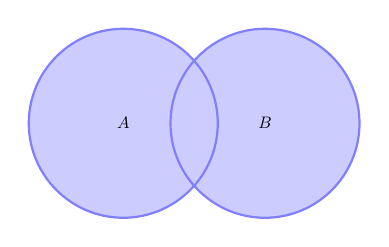
\begin{tikzpicture}[scale=0.6, every node/.style={scale=0.6}]
    \draw[filled] \firstcircle node {$A$}
                  \secondcircle node {$B$};
    %\node[anchor=south] at (current bounding box.north) {$A \cup B$};
\end{tikzpicture}
\end{center}

{\footnotesize
\begin{columns}
\begin{column}{0.3\textwidth}
left \\
\begin{tabular}{c|cc} \toprule
   & A  &  Key \\ \midrule
0 & A0 &  K0 \\
1 & A1 &  K1 \\ 
2 & A2 &  K2 \\
3 & A3 &  \textcolor{red}{K4} \\ \bottomrule
\end{tabular}
\vspace*{1.2em}
\end{column}
\begin{column}{0.27\textwidth}
right \\
\begin{tabular}{c|cc} \toprule
   &  B   & Key \\ \midrule
0 &  B0 & K0 \\
1 &  B1 & K1 \\ 
2 &  B2 & K2 \\
3 &  C3 & \textcolor{red}{K5} \\ \bottomrule
\end{tabular}
\vspace*{1.2em}
\end{column}
\begin{column}{0.3\textwidth}
merged \\
\begin{tabular}{c|ccc} \toprule
   & A  & B   & Key \\ \midrule
0 & A0 & B0 & K0 \\
1 & A1 & B1 & K1 \\ 
2 & A2 & B2 & K2 \\ 
3 & A3 & \textcolor{red}{NaN} & K4 \\ 
4 & \textcolor{red}{NaN} & B3 & K5 \\ \bottomrule
\end{tabular} \\
\vspace*{0.2em}
\end{column}
\end{columns}}

\end{frame}



\begin{frame}[containsverbatim]
\frametitle{Loop through DataFrames}

\lstinputlisting[language={Python}]{Codes/pandas-looping-01.py}

\begin{ausgabe}
K0 belongs to Anna
K1 belongs to Bernd
K2 belongs to Cesar
K4 belongs to Dana
\end{ausgabe}
\end{frame}

\section{Links}


\begin{frame}
\frametitle{Links}

\begin{itemize}
	\item \url{https://pandas.pydata.org/pandas-docs/stable/user_guide/10min.html}
	\item \url{https://pandas.pydata.org}
	\item 
	\item 
	\item 
	\item 
\end{itemize}



\end{frame}


\end{document}


\lstinline[style=Python]{input()}

